\documentclass[a4paper]{article}

%% Language and font encodings
\usepackage[english]{babel}
\usepackage[utf8x]{inputenc}
\usepackage[T1]{fontenc}

%% Sets page size and margins
\usepackage[a4paper,top=3cm,bottom=2cm,left=3cm,right=3cm,marginparwidth=1.75cm]{geometry}

%% Useful packages
\usepackage{amsmath}
\usepackage{float}
\usepackage{graphicx}
\usepackage{listings}
\usepackage{pgfplots}
\pgfplotsset{compat=1.14}
\usepackage[colorinlistoftodos]{todonotes}
\usepackage[colorlinks=true, allcolors=blue]{hyperref}
\graphicspath{ {./aipics/} }

\definecolor{dkgreen}{rgb}{0,0.6,0}
\definecolor{gray}{rgb}{0.5,0.5,0.5}
\definecolor{mauve}{rgb}{0.58,0,0.82}

\title{CS 440: Introduction to Artificial Intelligence}
\author{Brandon Smith \& Nicholas Grieco}

\begin{document}
\maketitle



\section*{Question 1: Optical Character Recognition}
\subsection{Partial Training Results}

Results when using 20\% to 100\% of the training data, when validating and testing on 1000 images.

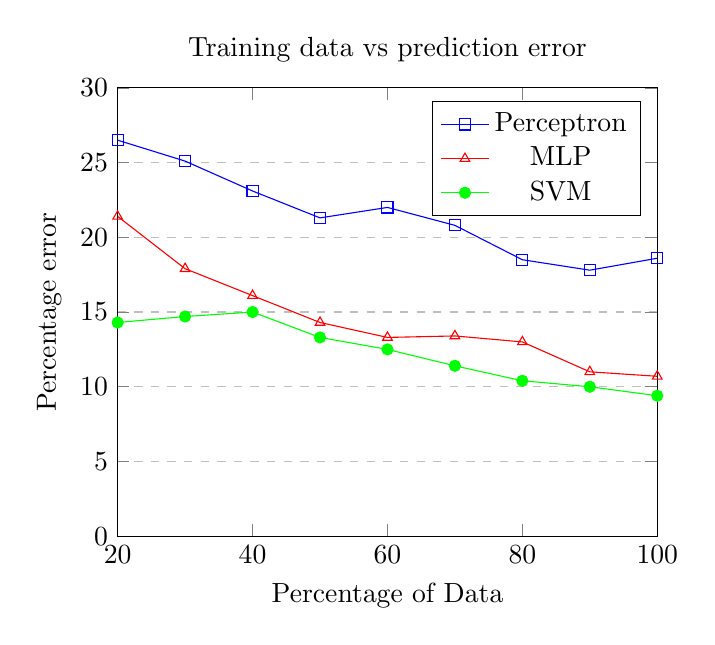
\begin{tikzpicture}
\begin{axis}[
    title={Training data vs prediction error},
    xlabel={Percentage of Data},
    ylabel={Percentage error},
    xmin=20, xmax=100,
    ymin=0, ymax=30,
    xtick={20,40,60,80,100},
    ytick={0,5,10,15,20,25,30},
    legend pos=north east,
    ymajorgrids=true,
    grid style=dashed,
]
 
\addplot[
    color=blue,
    mark=square,
    ]
    coordinates {
    (20,26.5)(30,25.1)(40,23.1)(50,21.3)(60,22)(70,20.8)(80,18.5)(90,17.8)(100,18.6)
    };
    
\addplot[
    color=red,
    mark=triangle,
    ]
    coordinates {
    (20,21.4)(30,17.9)(40,16.1)(50,14.3)(60,13.3)(70,13.4)(80,13)(90,11)(100,10.7)
    };
    
\addplot[
    color=green,
    mark=*,
    ]
    coordinates {
    (20,14.3)(30,14.7)(40,15)(50,13.3)(60,12.5)(70,11.4)(80,10.4)(90,10)(100,9.4)
    };
    
    \legend{Perceptron,MLP, SVM}
 
\end{axis}
\end{tikzpicture}

\subsection{Partial Testing Results}

Results when using 20\% to 100\% of the testing data, when training with 5000 images.

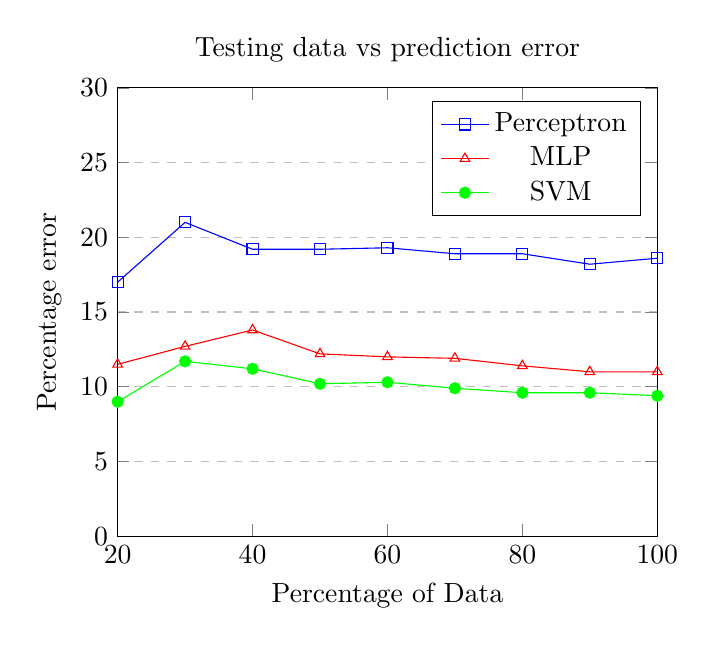
\begin{tikzpicture}
\begin{axis}[
    title={Testing data vs prediction error},
    xlabel={Percentage of Data},
    ylabel={Percentage error},
    xmin=20, xmax=100,
    ymin=0, ymax=30,
    xtick={20,40,60,80,100},
    ytick={0,5,10,15,20,25,30},
    legend pos=north east,
    ymajorgrids=true,
    grid style=dashed,
]
 
\addplot[
    color=blue,
    mark=square,
    ]
    coordinates {
    (20,17)(30,21)(40,19.2)(50,19.2)(60,19.3)(70,18.9)(80,18.9)(90,18.2)(100,18.6)
    };
    
\addplot[
    color=red,
    mark=triangle,
    ]
    coordinates {
    (20,11.5)(30,12.7)(40,13.8)(50,12.2)(60,12)(70,11.9)(80,11.4)(90,11)(100,11)
    };
    
\addplot[
    color=green,
    mark=*,
    ]
    coordinates {
    (20,9)(30,11.7)(40,11.2)(50,10.2)(60,10.3)(70,9.9)(80,9.6)(90,9.6)(100,9.4)
    };
    
    \legend{Perceptron,MLP, SVM}
 
\end{axis}
\end{tikzpicture}

\subsection{Qualitative Evaluation}
Hello
\section*{Question 2: University of Excellence}
\subsection*{a)} 
The provided tree is classified correctly.

\subsection*{b)}
GPA: $\geq$ 3.9, 3.2 < GPA < 3.9 , $\leq$ 3.2\\
Research: Yes, No\\
Rank: 1, 2, 3\\

\underline{Level 1}

\begin{tabular}{ |p{3cm}||p{3cm}|p{3cm}| }
 \hline
 \multicolumn{3}{|c|}{GPA} \\
 \hline
 & Positive & Negative\\
 \hline
 $\geq 3.9$  & 3 & 0\\
 3.2 < GPA < 3.9 &   3 & 2\\
 $\leq 3.2$ & 0 & 4\\
 \hline
\end{tabular}

Remainder = $\frac{3}{12}$ B(1) + $\frac{5}{12}$ B($\frac{3}{5}$)  + $\frac{1}{3}$ B(0)= 0.4046\\

\begin{tabular}{ |p{3cm}||p{3cm}|p{3cm}| }
 \hline
 \multicolumn{3}{|c|}{Research} \\
 \hline
 & Positive & Negative\\
 \hline
 Yes & 3 & 2\\
 No &   3 & 4\\
 \hline
\end{tabular}

Remainder = $\frac{5}{12}$ B($\frac{3}{5}$) + $\frac{7}{12}$ B($\frac{3}{7}$) = 0.9792\\

\begin{tabular}{ |p{3cm}||p{3cm}|p{3cm}| }
 \hline
 \multicolumn{3}{|c|}{Rank} \\
 \hline
 & Positive & Negative\\
 \hline
 Rank 1 & 3 & 2\\
 Rank 2 &   2 & 1\\
 Rank 3 &   1 & 3\\
 \hline
\end{tabular}

Remainder = $\frac{5}{12}$ B($\frac{3}{5}$) + $\frac{1}{4}$ B($\frac{2}{3}$)  + $\frac{1}{3}$ B($\frac{1}{4}$)= 0.9046\\

\begin{tabular}{ |p{3cm}||p{3cm}|p{3cm}| }
 \hline
 \multicolumn{3}{|c|}{Reccomendation} \\
 \hline
 & Positive & Negative\\
 \hline
 Good & 5 & 3\\
 Normal &   1 & 3\\
 \hline
\end{tabular}

Remainder = $\frac{8}{12}$ B($\frac{5}{8}$) + $\frac{4}{12}$ B($\frac{1}{4}$) = 0.9067\\

\textbf{GPA} has the lowest remainder so we choose that option for the first level.

\underline{Level 2}

\begin{tabular}{ |p{3cm}||p{3cm}|p{3cm}| }
 \hline
 \multicolumn{3}{|c|}{Research} \\
 \hline
 & Positive & Negative\\
 \hline
 Yes & 2 & 0\\
 No &   1 & 2\\
 \hline
\end{tabular}

Remainder = $\frac{2}{5}$ B(1) + $\frac{3}{5}$ B($\frac{1}{3}$) = 0.5510\\

\begin{tabular}{ |p{3cm}||p{3cm}|p{3cm}| }
 \hline
 \multicolumn{3}{|c|}{Rank} \\
 \hline
 & Positive & Negative\\
 \hline
 Rank 1 & 1 & 1\\
 Rank 2 &   1 & 0\\
 Rank 3 &   1 & 1\\
 \hline
\end{tabular}

Remainder = $\frac{2}{5}$ B(1) +  B(1) + $\frac{2}{5}$ B($\frac{1}{2}$) = 0.80\\

\begin{tabular}{ |p{3cm}||p{3cm}|p{3cm}| }
 \hline
 \multicolumn{3}{|c|}{Reccomendation} \\
 \hline
 & Positive & Negative\\
 \hline
 Good & 3 & 2\\
 Normal &   0 & 0\\
 \hline
\end{tabular}

Remainder = B($\frac{3}{5}$) +  B(1) + B(1) = 0.9710\\

\textbf{Research} has the lowest remainder so we choose that option for the second level.

\underline{Level 3}

\begin{tabular}{ |p{3cm}||p{3cm}|p{3cm}| }
 \hline
 \multicolumn{3}{|c|}{Rank} \\
 \hline
 & Positive & Negative\\
 \hline
 Rank 1 & 0 & 1\\
 Rank 2 &   1 & 0\\
 Rank 3 &   0 & 1\\
 \hline
\end{tabular}

Remainder = B(1) +  B(1) + B(1) = 0\\

\begin{tabular}{ |p{3cm}||p{3cm}|p{3cm}| }
 \hline
 \multicolumn{3}{|c|}{Reccomendation} \\
 \hline
 & Positive & Negative\\
 \hline
 Good & 1 & 2\\
 Normal &   0 & 0\\
 \hline
\end{tabular}

Remainder =B(1) + B($\frac{1}{3}$) = 0.9183\\

\textbf{University ranking} has the lowest remainder so we choose that option for the last level.

\subsection*{c)}
Yes they classify the same way because it's the same tree. It is not a coincidence. At each state the best attribute was chosen. The only time you can have different trees from the same data is at any given 2 attributes have the same remainder and you can choose.
\section*{Question 3: SVM}
Question 3 goes here
\section*{Question 4: Perceptrons}



\subsection*{a)}
\begin{figure}[H]
\caption{Single Perceptron}
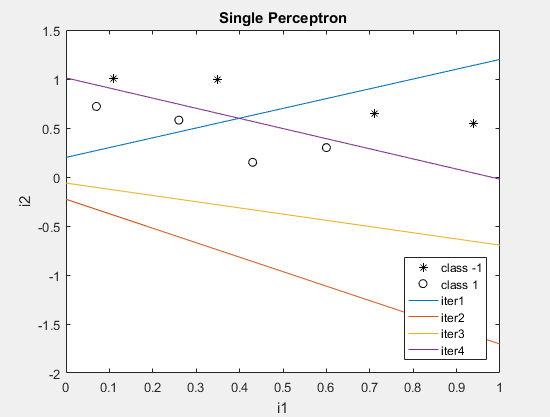
\includegraphics[width=8cm]{singleperc.png}
\centering
\end{figure}

\lstset{frame=tb,
  language=Python,
  aboveskip=3mm,
  belowskip=3mm,
  showstringspaces=false,
  columns=flexible,
  basicstyle={\small\ttfamily},
  numbers=none,
  numberstyle=\tiny\color{gray},
  keywordstyle=\color{blue},
  commentstyle=\color{dkgreen},
  stringstyle=\color{mauve},
  breaklines=true,
  breakatwhitespace=true,
  tabsize=3
}

\begin{lstlisting}[float=h,frame=tb,caption=Perceptron Code,label=zebra]
from random import choice
from numpy import array, dot, random

unit_step = lambda x: -1 if x < 0 else 1

training_data = [
    (array([1,0.1,0.72]), -1),
    (array([1,0.15,1.01]), 1),
    (array([1,0.25,0.55]), -1),
    (array([1,0.32,0.95]), 1),
    (array([1,0.45,0.12]), -1),
    (array([1,0.6,0.3]), -1),
    (array([1,0.7,0.6]), 1),
    (array([1,0.9,0.4]), 1),
]

w = [0.2, 1, -1]
errors = []
eta = 1
epoch = 5

print("Initial Weights: " + str(w))
for z in range(epoch):
    print("Epoch: " + str(z + 1))
    for i in xrange(len(training_data)):
        x, expected = training_data[i]
        result = dot(w, x)
        error = expected - unit_step(result)
        errors.append(error)
        w += eta * error * x
    print("Updated weights: " + str(w))
    tmp_err = 0
    for l in range(len(training_data)):
        x, expected = training_data[l]
        result = dot(w, x)
        if expected != unit_step(result):
            tmp_err = tmp_err + 1
    print("Missclassified: " + str(tmp_err))
\end{lstlisting}

\begin{lstlisting}[float=h,frame=tb,caption=Code output,label=zebra]
Epoch: 1
Updated weights: [ 0.2   1.3   0.88]
Missclassified: 4
Epoch: 2
Updated weights: [ 0.2   2.04  3.22]
Missclassified: 4
Epoch: 3
Updated weights: [-1.8   1.84  1.78]
Missclassified: 0
Epoch: 4
Updated weights: [-1.8   1.84  1.78]
Missclassified: 0
\end{lstlisting}

By iteration 4 all the points were being perfectly classified.

\clearpage
\subsection*{b)}
The perceptron perfectly classified the set of points.

\subsection*{c)}

\begin{figure}[H]
\caption{Single layer perceptrons}
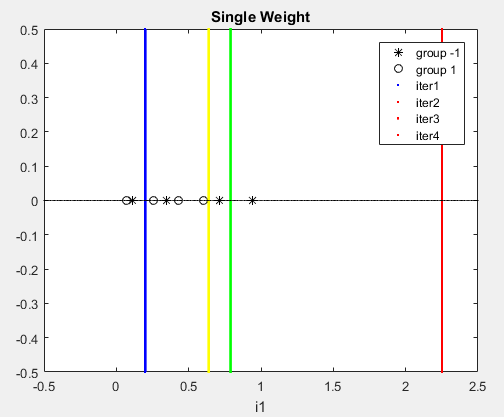
\includegraphics[width=8cm]{svmlin.png}
\centering
\end{figure}

The best we can linearly separate the data points without $i_2$ is 2 classification errors. 
We get $b = -1.8$ and $w_1 = 2.82$ making the point it separates at $i_0$ = 0.63 
\section*{Question 5: Classification}

\subsection*{a)}
\begin{figure}[H]
\caption{Single layer perceptrons}
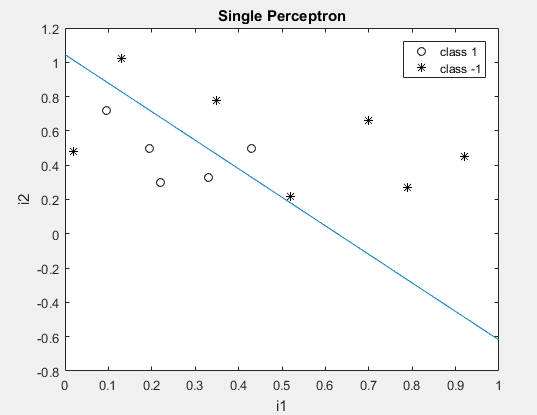
\includegraphics[width=8cm]{singlenonlin.png}
\centering
\end{figure}

Using the same code for the perceptron as in question 4, I was able to get a minimum of 2 classification errors. This means the data points are non-linearly separable. A multi-layer perceptron would be better in classifying this set of data.



\subsection*{b)}

\begin{figure}[H]
\caption{Multi layer perceptrons}
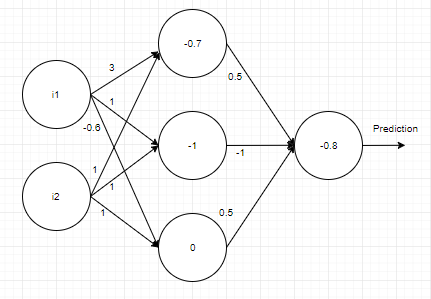
\includegraphics[width=8cm]{hidden.png}
\centering
\end{figure}

\begin{figure}[H]
\caption{Dividing lines of multi layer perceptron}
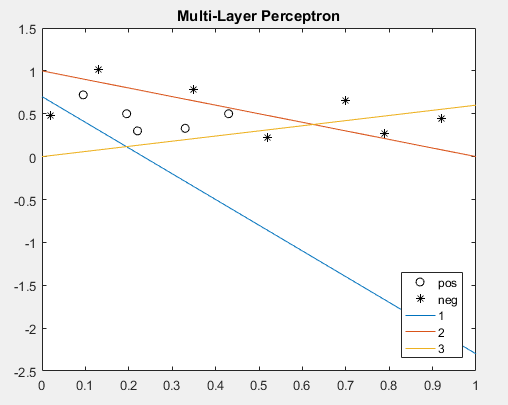
\includegraphics[width=8cm]{q5mlp.png}
\centering
\end{figure}

$w_{11} = 3, w_{12} = 1, w_{13} = -0.6$\\
$w_{21} = 1, w_{22} = 1, w_{23} = 1$\\
$b_1 = -0.7, b_2 = -1, b_3 = 0, b_4 = -0.8$\\

\end{document}